\section{Understanding Bipartite Networks}

\begin{frame}
\frametitle{Why Early-Late Stage Distinction Matters}

\begin{columns}
\begin{column}{0.5\textwidth}
\textbf{Early-Stage Investors}
\begin{itemize}
    \item Focus on \textbf{seed \& Series A}
    \item Higher risk tolerance
    \item Hands-on mentoring
    \item Smaller investment amounts
    \item Technology \& market validation
\end{itemize}
\end{column}

\begin{column}{0.5\textwidth}

\textbf{Late-Stage Investors}
\begin{itemize}
    \item Focus on \textbf{Series B+}
    \item Growth capital orientation
    \item Scaling expertise
    \item Larger investment amounts
    \item Market expansion \& profitability
\end{itemize}
\end{column}
% \begin{column}{0.45\textwidth}
% \begin{figure}
%     \centering
%     
\includegraphics[width=\textwidth]{../figures/us/investment_stage_distribution.png}
%     \caption{Investment stage distribution}
% \end{figure}
% \end{column}
\end{columns}

\begin{alertblock}{Key Insight}
These different roles justify modeling them as \textbf{separate node types} in a bipartite network!
\end{alertblock}

\end{frame}

\begin{frame}
\frametitle{From Classical to Bipartite Syndication Models}

\begin{figure}
    \centering
    
\includegraphics[width=0.9\textwidth]{../figures/diagrams/classical_syndication_net.png}
    \caption{Classical syndication model. All investors treated equally}
\end{figure}

\begin{itemize}
    \item Traditional approach: connect all co-investors equally
    \item \textbf{Problem}: obscures role differentiation and hierarchical patterns
    \item \textbf{Our solution}: bipartite representation preserving investor roles
\end{itemize}

\end{frame}

\begin{frame}
\frametitle{Unipartite vs. Bipartite Network Representations}

\begin{columns}
  \begin{column}{0.6\textwidth}
    \begin{figure}
      \centering
      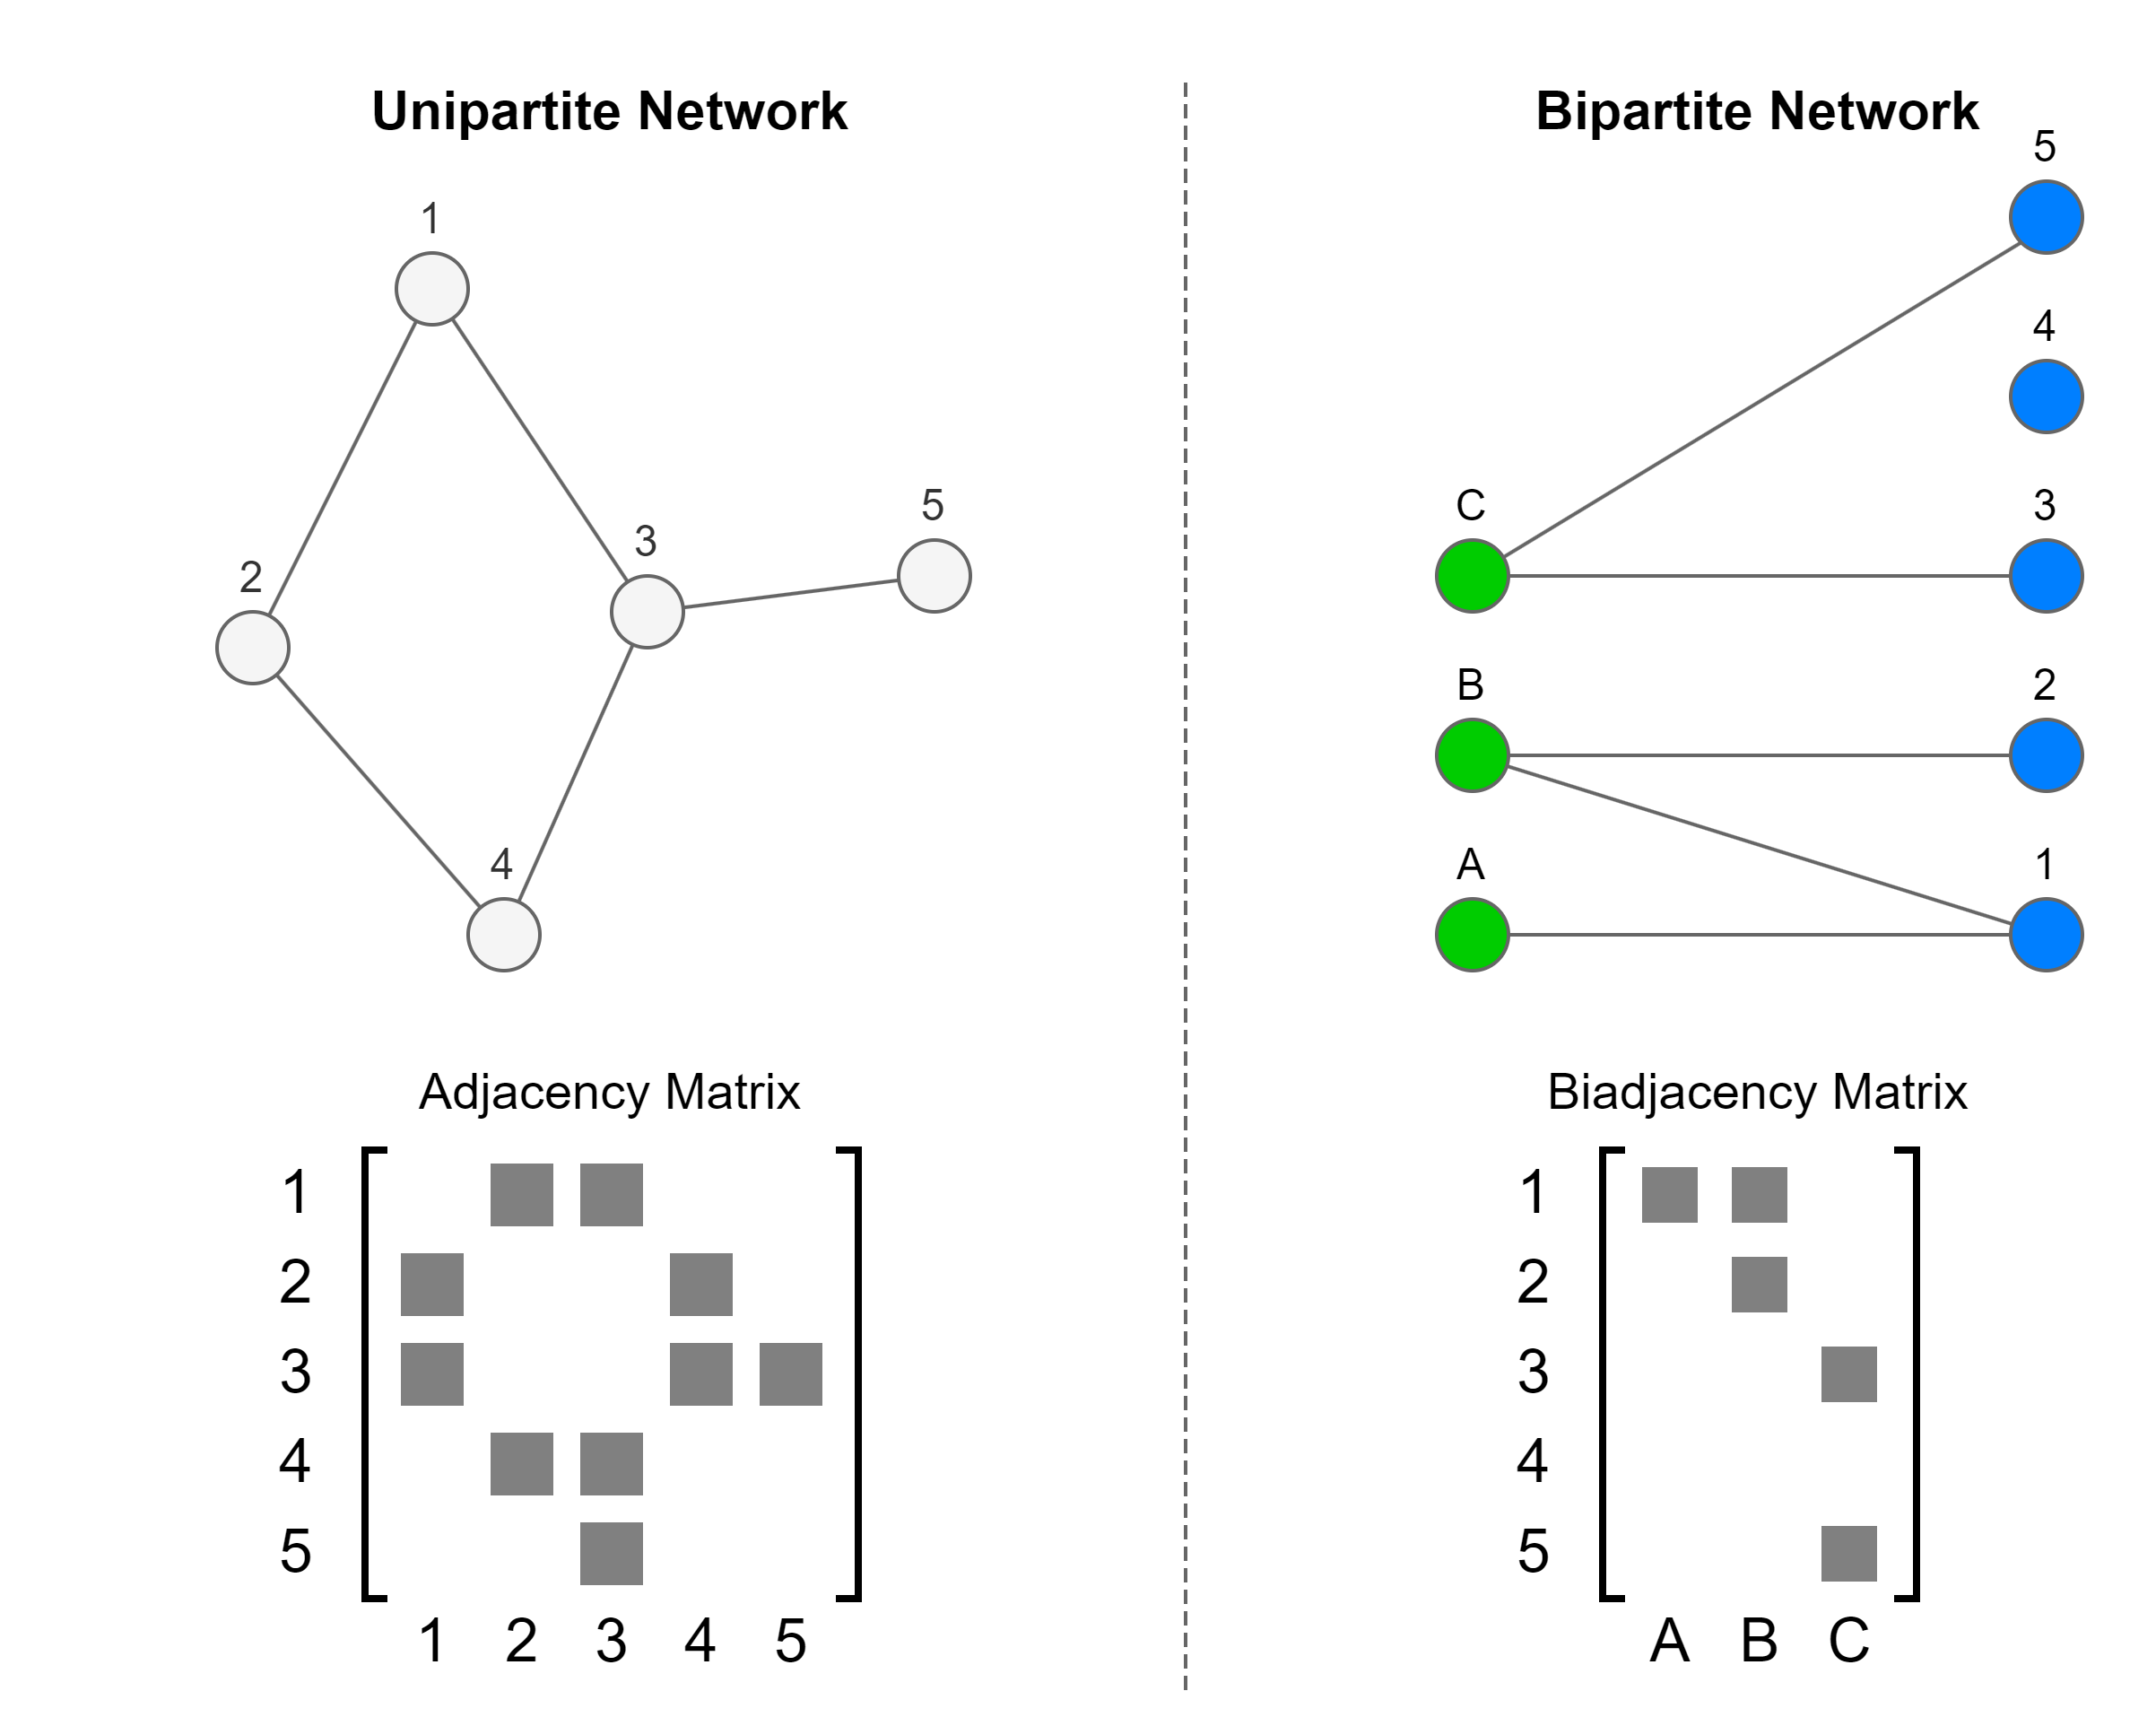
\includegraphics[width=\textwidth]{../figures/diagrams/unipartite_vs_bipartite_networks_v2.png}
      % \caption{Key differences in network structure and matrix representation}
    \end{figure}
  \end{column}
  \begin{column}{0.4\textwidth}
    \begin{itemize}
      \item \textbf{Unipartite}: Single node set, square adjacency matrix
      \item \textbf{Bipartite}: Two disjoint node sets, rectangular biadjacency matrix
      \item Bipartite structure \textbf{essential} for detecting nestedness patterns
    \end{itemize}
  \end{column}
\end{columns}

\end{frame}

\begin{frame}
\frametitle{Our Early-Late Stage Bipartite Model}

\begin{figure}
    \centering
    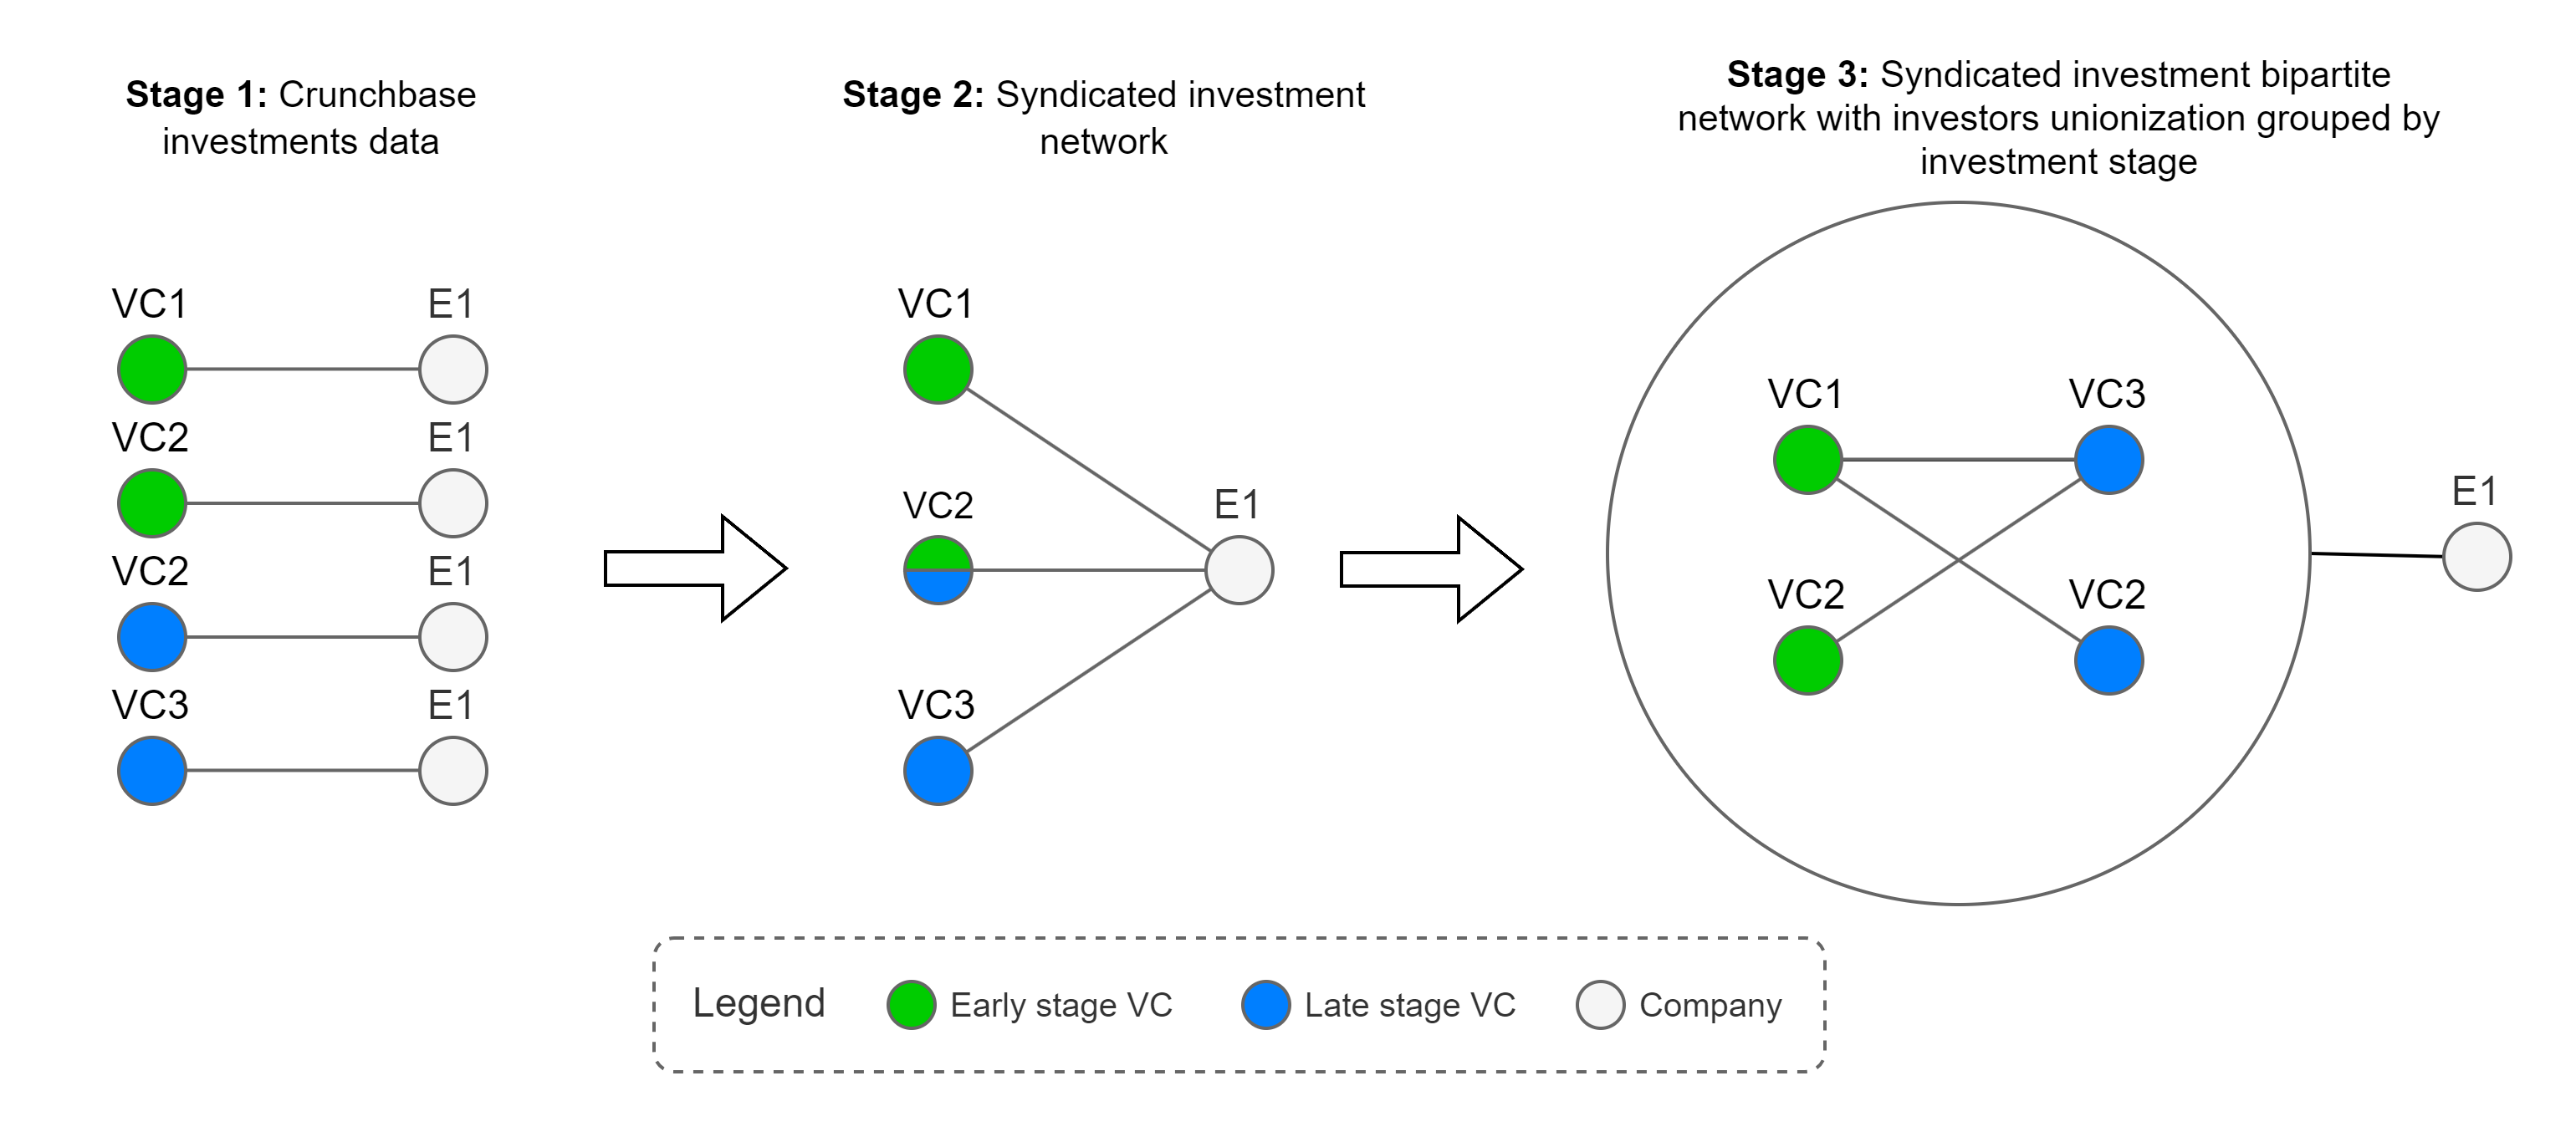
\includegraphics[width=0.9\textwidth]{../figures/diagrams/vc_investment_bipartite_pipeline.png}
    % \caption{Construction pipeline: from investment events to bipartite network}
\end{figure}

\begin{itemize}
    \item Early-stage investors $\leftrightarrow$ Late-stage investors
    \item Edges = co-investment in same companies
    \item Preserves sequential flow of capital across funding stages
    \item Enables analysis of hierarchical organization patterns
\end{itemize}

\end{frame}
